\documentclass{article}
\usepackage[utf8]{inputenc}
\usepackage{amsmath}
\usepackage{amsfonts}
\usepackage{multirow}
\usepackage[table]{xcolor}
\usepackage{amsthm}%
\usepackage{mathtools}
%\usepackage{mathdesign}
\usepackage{mathrsfs}
\usepackage{graphicx}
\usepackage{algorithmicx}
%\usepackage{algorithmic}
%\usepackage{ctmmath-v2}
%\setlength{\arrayrulewidth}{1mm}
%\setlength{\tabcolsep}{18pt}
%\renewcommand{\arraystretch}{2.5}



%\documentclass{beamer}

%\usepackage{unicode-math}
\usepackage[utf8]{inputenc}
\usepackage{amsmath}
\usepackage{amsfonts}
\usepackage{multirow}
\usepackage{mathtools}
\usepackage{mathdesign}
\usepackage{mathrsfs}
\usepackage{graphicx}
\usepackage{amsthm}%
\usepackage[table]{xcolor}
\setlength{\arrayrulewidth}{1mm}
\setlength{\tabcolsep}{18pt}
\renewcommand{\arraystretch}{2.5}

\newcolumntype{s}{>{\columncolor[HTML]{AAACED}} p{2cm}}
\arrayrulecolor[HTML]{DB5800}


%graphics paths
\graphicspath{{./home/charles/Documents/tex/2Phase/figures}{./figures}{/figures}{home/chaztikov/git/nldt/pythonc/05232019/}}




%new commands
\newcommand{\vol}{\mathfrak{vol}}
\newcommand{\baba}[1]{\overline{\overline{#1}}}
\newcommand{\mean}[1]{\left\langle #1 \right\rangle} 
\newcommand{\iavg}[2]{{\mean{#1}}_{#2}}
\newcommand{\iiavg}[2]{{\iavg{#1}{#2}}_{#2}}
%\newcommand{\iiavg}[2][2]{{\mean{#1}}_{{#2}{#2}}}
%\newcommand{\iiiavg}[4]{{\iiavg{#1}{#2}{#2}{#4}}}
\newcommand{\mb}[1]{\mathbf{#1}}
\newcommand{\norm}[1]{\left \|  #1 \right \|}




\begin{document}
	
\section{Data}

\begin{figure}
	\centering
	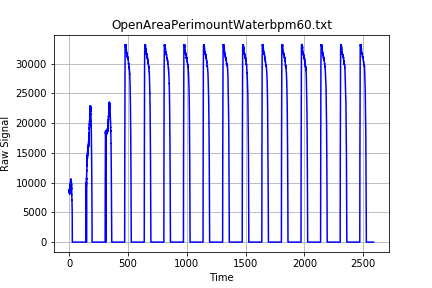
\includegraphics[width=0.7\linewidth]{raw_0}\includegraphics[width=0.7\linewidth]{raw_1}
	\includegraphics[width=0.7\linewidth]{raw_2}\includegraphics[width=0.7\linewidth]{raw_3}
	\caption{Raw Signal Data}
	\label{fig:raw0}
\end{figure}
%
%\begin{figure}
%	\centering
%	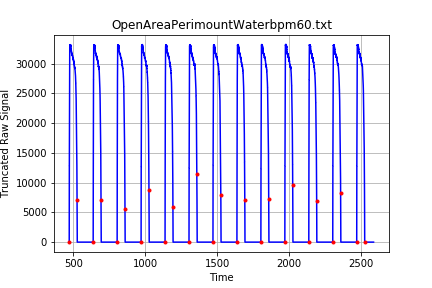
\includegraphics[width=0.7\linewidth]{truncraw_0}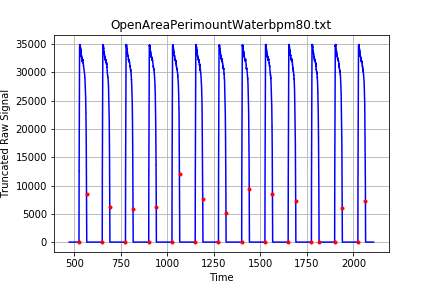
\includegraphics[width=0.7\linewidth]{truncraw_1}
%	\includegraphics[width=0.7\linewidth]{truncraw_2}\includegraphics[width=0.7\linewidth]{truncraw_3}
%	\caption{Raw Signal Data}
%	\label{fig:raw0}
%\end{figure}

%
%\includegraphics[width=0.7\linewidth]{home/chaztikov/git/nldt/pythonc/05232019/raw_1}	\includegraphics[width=0.7\linewidth]{home/chaztikov/git/nldt/pythonc/05232019/raw_2}	\includegraphics[width=0.7\linewidth]{home/chaztikov/git/nldt/pythonc/05232019/raw_3}
\begin{figure}
	\centering
	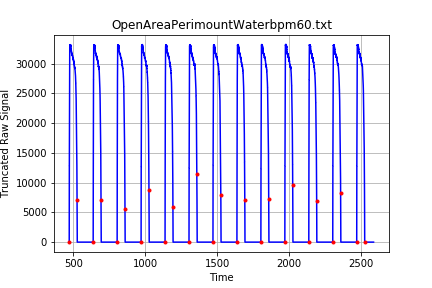
\includegraphics[width=0.7\linewidth]{truncraw_0}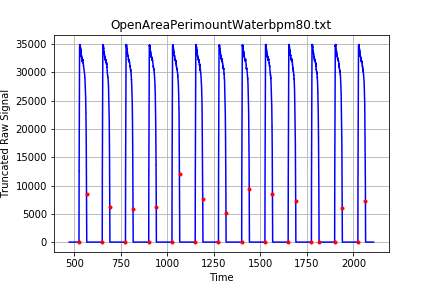
\includegraphics[width=0.7\linewidth]{truncraw_1}
	\caption{Truncated Raw Signal Data (aligned at red points)}
	\label{fig:truncraw0}
\end{figure}

\begin{figure}
	\centering
	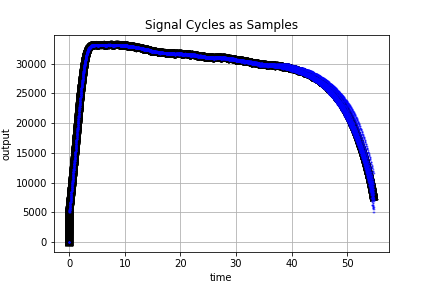
\includegraphics[width=0.7\linewidth]{mean_0}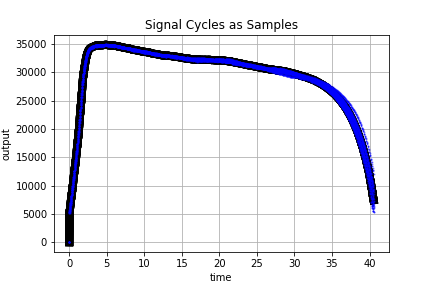
\includegraphics[width=0.7\linewidth]{mean_1}
	\caption{Signal Mean (black) from samples (blue)}
	\label{fig:mean0}
\end{figure}

\begin{figure}
	\centering
	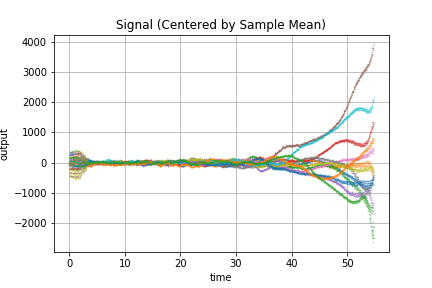
\includegraphics[width=0.7\linewidth]{centered_0}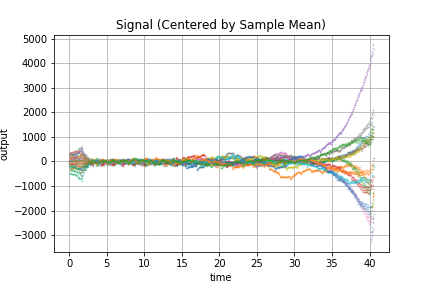
\includegraphics[width=0.7\linewidth]{centered_1}
	\caption{Centered Signals}
	\label{fig:centered0}
\end{figure}
%
%\begin{figure}
%	\centering
%	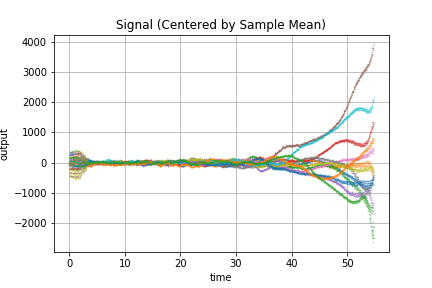
\includegraphics[width=0.7\linewidth]{centered_0}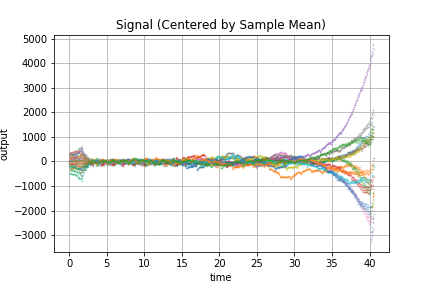
\includegraphics[width=0.7\linewidth]{centered_1}
%	\caption{Centered Signals}
%	\label{fig:centered0}
%\end{figure}


\begin{figure}
	\centering
	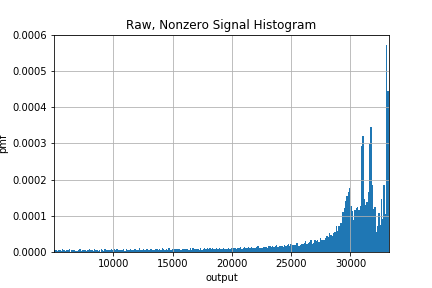
\includegraphics[width=0.7\linewidth]{histnz_0}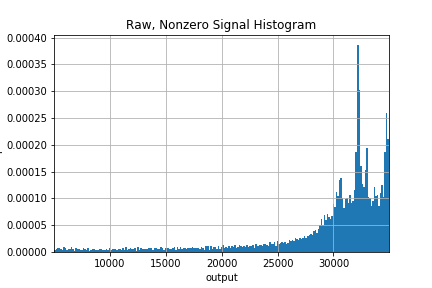
\includegraphics[width=0.7\linewidth]{histnz_1}
	\caption{}
	\label{fig:histnz0}
\end{figure}


\section{PCA}

\subsection{Truncated Transient, Waves as Samples}

\begin{figure}
	\centering
	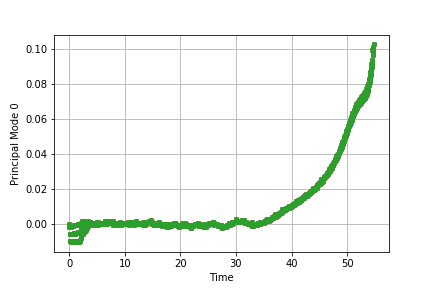
\includegraphics[width=0.7\linewidth]{pca_pm2pm0}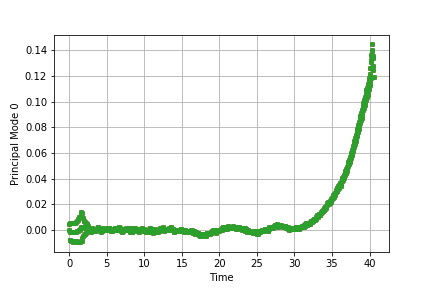
\includegraphics[width=0.7\linewidth]{1_pca_pm2pm0}	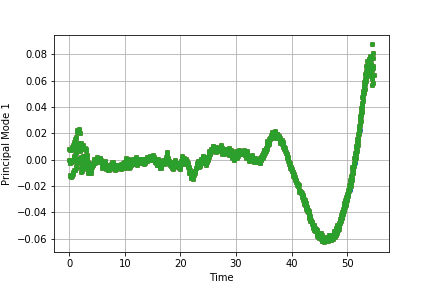
\includegraphics[width=0.7\linewidth]{pca_pm2pm1}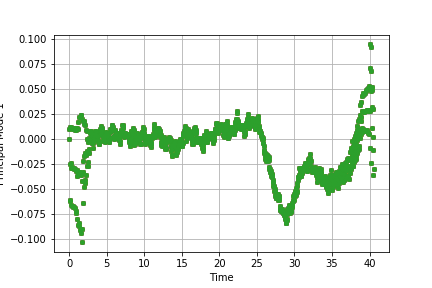
\includegraphics[width=0.7\linewidth]{1_pca_pm2pm1}
	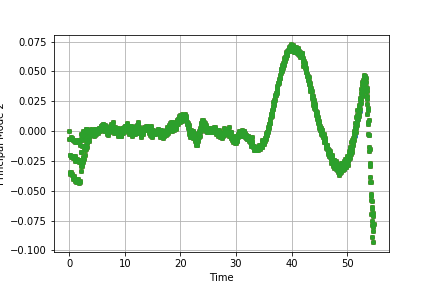
\includegraphics[width=0.7\linewidth]{pca_pm2pm2}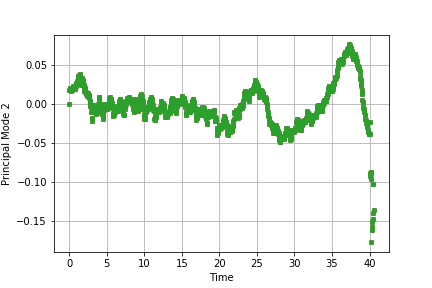
\includegraphics[width=0.7\linewidth]{1_pca_pm2pm2}
	\caption{Principal Modes 1,2,3 (rows) for two datasets (columns)}
	\label{fig:1pcapm2pm0}
\end{figure}




\begin{figure}
	\centering
	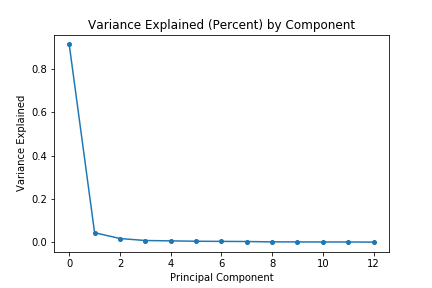
\includegraphics[width=0.7\linewidth]{0_pca_explained_variance_ratio_}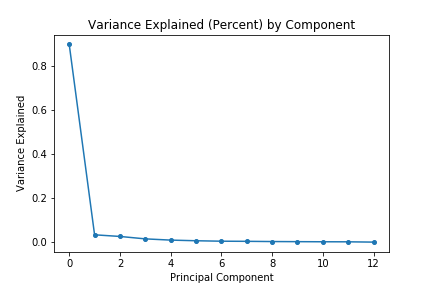
\includegraphics[width=0.7\linewidth]{1_pca_explained_variance_ratio_}
	\caption{Explained Variance Ratio}
	\label{fig:0pcaexplainedvarianceratio}
\end{figure}





















\section{Factor Analysis}

\begin{figure}
	\centering
	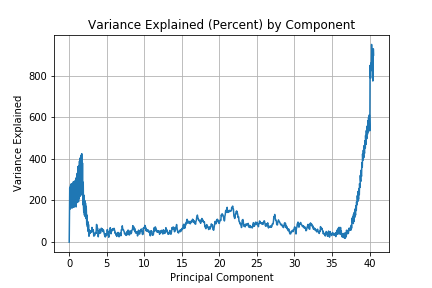
\includegraphics[width=0.7\linewidth]{1_fa_explained_variance_ratio_}
	\caption{Factor Analysis time-dependent noise variance (red and green) by }
	\label{fig:1faexplainedvarianceratio}
\end{figure}

\begin{figure}
	\centering
	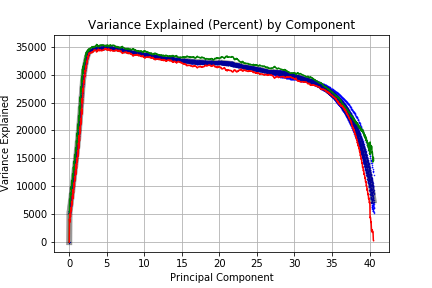
\includegraphics[width=0.7\linewidth]{1_fa_bands_}
	\caption{Factor Analysis procures Bounds by determined time-dependent noise variance (red and green) by }
	\label{fig:1fabands}
\end{figure}


\subsection{Truncated Transient, Waves as Samples}



\section{References}

\end{document}